\begin{enumerate}[A]
	\item 轴的受力分析
	\begin{enumerate}[a]
		\item 画受力简图
		\par 圆周力 $$F_t=\frac{2T_{\mathrm{{\uppercase\expandafter{\romannumeral1}}}}}{d}=1215.44$$
		径向力 $$F_r=F_t\tan{20^{\circ}}=442.38$$
		\item 计算支反力 
		\begin{figure}[H]
			\begin{center}
				\caption{轴\uppercase\expandafter{\romannumeral1}的支反力图}
				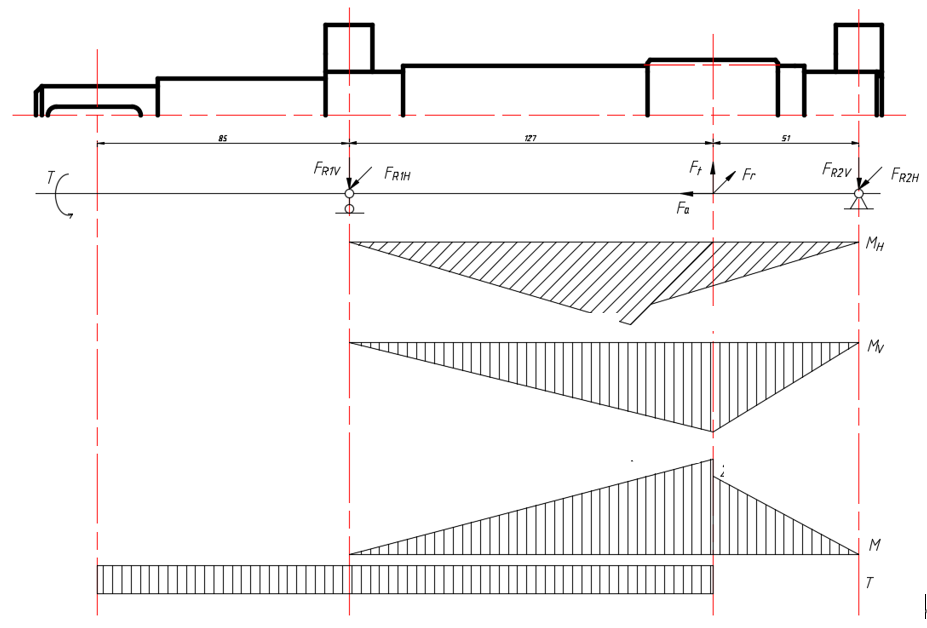
\includegraphics[width=\textwidth]{pic/jiaohe1.png}
			\end{center}
		\end{figure}
		\par 在水平面上:
		$$F_{R1H}=\dfrac{F_r\cdot C_1+F_a\cdot \dfrac{d}{2}}{B_1+C_1}=218.97$$
		$$F_{R2H}=F_r-F_{R1H}=223.41$$
		\par 在垂直平面上:
		$$F_{R1V}=\dfrac{F_t\cdot C_1}{B_1+C_1}=601.61$$
		$$F_{R2V}=F_t-F_{R1V}=613.83$$
		轴承1的总的支反力为
		$$F_{R1}=\sqrt{{F_{R1H}}^2+{F_{R1V}}^2}=640.22$$
		轴承2的总的支反力为
		$$F_{R2}=\sqrt{{F_{R2H}}^2+{F_{R2V}}^2}=653.22$$
		\item 画弯矩图
		\par 在水平面上 \\
		a-a剖面线左侧\\
		$$M_{aH}=F_{R1H}B_1=22006.49$$
		a-a剖面右侧 \\
		$$M^{\prime}_{aH}=F_{R2H}C_1=22005.89$$
		垂直面上,弯矩为\\
		$$M_{aH}=F_{R1V}B_1=60461.81$$
		合成弯矩\\
		a-a剖面左侧\\
		$$M_a=\sqrt{{M_{aH}}^2+{M_{aV}}^2}=64342.18$$
		a-a剖面右侧\\
		$$M^{\prime}_a=\sqrt{{M^{\prime}_{aH}}^2+{M_{aV}}^2}=64341.97$$
		
		\item 画转矩图$$T=1.704\times 10^4$$
	\end{enumerate}
	\item 校核轴的强度
	\par a-a剖面左侧的弯曲强度大,有转矩,为危险截面。
	\par 该截面抗弯模量为
	$$W=0.1{d_5}^3-\dfrac{bt\left(d_5-t\right)^2}{2d_5}=2667.7$$
	该截面的抗扭截面模量为
	$$W_T=0.2{d_5}^3-\dfrac{bt\left(d_5-t\right)^2}{2d_5}=5335$$
	弯曲应力$$\sigma_b=\dfrac{M}{W}=24.12$$
	$$\sigma_a=\sigma_b=24.12$$
	$$\sigma_m=0$$
	扭剪应力
	$$\tau_T=\dfrac{T}{W_T}=3.194$$
	$$\tau_a=\tau_m=\dfrac{\tau_T}{2}=1.60$$
	\par 调质处理的45钢,由参考文献\cite{2}表9.3可以查得$\sigma_b=650$,$\sigma_{-1}=300$,$\tau_{-1}=155$;材料等效系数$\psi_\sigma=0.2$,$\psi_\tau=0.1$。
	\par 因为是齿轮轴无键槽,取$K_\sigma=1$,$K_\tau=1$。
	\par 查参考文献\cite{2}表9.12得$\epsilon_\sigma=0.88$,$\epsilon_\tau=0.81$。
	\par 查参考文献\cite{2}表9.9得$\beta=1$。
	\par 由此,安全系数计算如下:
	$$S_\sigma=\dfrac{\sigma_{-1}}{\dfrac{K_\sigma}{\beta \epsilon_\sigma}\sigma_a+\psi_\sigma \sigma_m}=10.94$$
	$$S_\tau=\dfrac{\tau_{-1}}{\dfrac{K_\tau}{\beta \epsilon_\tau}\tau_a+\psi_\tau \tau_m}=72.59$$
	$$S=\dfrac{S_\sigma\cdot S_\tau}{\sqrt{{S_\sigma}^2+{S_\tau}^2}}=10.82$$
	\par 由参考文献\cite{2}表9.13得许用安全系数$\left[S\right]=1.3\sim 1.5$,显然$S>\left[S\right]$,故a-a截面安全。
	
	\item 校核键连接的强度
	\par 键连接的挤压应力\\$$\sigma_p=\dfrac{4T}{dhl}$$
	式中:d——键连接处的轴径,mm;\\
	T——传递的转矩,$\mathrm{N}\cdot \mathrm{mm}$;\\
	h——键的高度,mm;\\
	l——键连接长度,mm;
	\par 故联轴器处键连接的挤压应力为$$\sigma_p=\dfrac{4T}{dhl}=13.71$$
	\par 键、轴材料均为45钢,$\left[\sigma_p\right]= 120~150$。$\sigma_p<\left[\sigma_p\right]$,故强度满足需要。
	\item 校核轴承强度
	\par 由参考文献\cite{1}表12.4查得6205轴承的$C_r=14000$,$C_0=7880$。
	\begin{enumerate}[a]
		\item 计算轴承的轴向力
		\par 由于是深沟球轴承和圆柱齿轮,所以轴向力不予考虑。所以需要同时校核轴承1和2。
		\item 计算当量动载荷
		\par 由于是深沟球轴承和圆柱齿轮,所以无需计算当量动载荷,只需计算轴承寿命。
		\item 校核轴承寿命
		\begin{itemize}
			\item 校核轴承1的寿命
			\par 轴承在\SI{100}{\degreeCelsius}下工作,$f_T=1$。根据其载荷性质,取$f_F=1.2$。又由于是深沟球轴承、直齿轮,故$F_1=F_{R1}$,$F_2=F_{R2}$。
			\par 轴承寿命为
			$$L_h=\dfrac{10^6}{60n_{\mathrm{\uppercase\expandafter{\romannumeral1}}}}{\left(\dfrac{f_tC_r}{f_FF_{R1}}\right)}^3=71025.30$$
			\par 已知减速器使用年限为五年两班工作制,则预期寿命为
			$${L_h}^{\prime}=8\times 2\times 250\times 5=20000$$
			故轴承的寿命很充裕
			\item 校核轴承2的寿命
			\par 轴承在\SI{100}{\degreeCelsius}下工作,$f_T=1$。根据其载荷性质,取$f_F=1.2$。
			\par 轴承寿命为
			$$L_h=\dfrac{10^6}{60n_{\mathrm{\uppercase\expandafter{\romannumeral1}}}}{\left(\dfrac{f_tC_r}{f_FF_{R2}}\right)}^3=66868.62$$
			\par 已知减速器使用年限为五年两班工作制,则预期寿命为
			$${L_h}^{\prime}=8\times 2\times 250\times 5=20000$$
			故轴承的寿命很充裕
		\end{itemize}
	\end{enumerate}
\end{enumerate}